\documentclass[twoside]{wiss}

\usepackage{ascmac}
\usepackage[dvipdfmx]{graphicx}
\usepackage[balance]{nidanfloat}
\usepackage{multicol}
\usepackage{color}
\usepackage{url}

\journalhead{PLATEAUを用いた街模型製作支援ツールキットの開発}

\begin{document}

\title{PLATEAUを用いた街模型製作支援ツールキットの開発}
\etitle{}
\author{青嶋 勇太\affil{東京電機大学}　　岩井 将行${}^*$}

\begin{abstract}
本研究では，空間データを直感的に解釈するためのData Physicalizationに着目し，3D都市モデル（PLATEAU）と各種データを統合するフィジカルデバイス制作支援ツールキット「machimoki」を提案する．防災情報の立体化や街作りIoT環境センシング等，空間データの理解には立体形状が極めて有効である．しかし従来の立体模型製作は，オープンデータの抽出・加工，3Dプリントに適したソリッドモデル化，さらに内部への電子部品組み込みなど高度な専門性を要し，試作の難易度が高かった．本システムでは，Web地図上での領域指定のみでPLATEAU建物と地形を統合したソリッドモデルを自動生成し，LEDやセンサを組み込むフィジカルコンピューティング制作を一貫支援する．本稿では，浸水シミュレーションや環境センシングを対象とした試作例を示すとともに，物理模型と画面が相互連動するプロトタイプシステムの設計と動作について報告する．
\end{abstract}


\maketitle

\section{はじめに}
近年，IoTセンサデータや防災ハザード情報の活用が進む一方，従来の平面画面を介した可視化（Digital Twin）では，建物の立体的な密集度や地形の高低差を伴う空間的な直感把握，住民協議等における協調的な議論において限界が存在する．これに対し，データを物理的な実体として表現し空間的直感を活用する「Data Physicalization」\cite{jansen2015}が注目されている．国土交通省の「Project PLATEAU」\cite{plateau}等の公開により高精度な3D都市データが利用可能となったが，実プリント可能なソリッドモデル（閉じたメッシュ）の製作や電子部品の組み込みには，(1)~広大な3Dデータからの領域抽出と縮尺変換，(2)~底面開口や自己交差のないソリッド化，(3)~配線・センサ配置用設計，という高い技術障壁が存在する．

そこで本研究では，Webブラウザ上の地図操作のみでPLATEAU建物・地形データを統合し，3Dプリント可能なソリッドモデルを自動生成するとともに，LEDやセンサを組み込む制作を一貫支援するツールキット「machimoki」を提案する．

\section{関連研究}
Data Physicalizationにおいて，3Dプリント模型へのプロジェクションマッピングやLED配置による情報提示手法が提案されてきた．しかし，従来手法の多くは専門的なGIS・3Dモデリングツールを用いた手作業に依存しており，一般の開発者や市民が独自の模型を製作することは困難であった．また回路・センサ組み込み構造を自動生成するファブリケーション支援研究も存在するが，オープンな3D都市モデルと連携し，Web上で領域選択からソリッドモデル化，IoT組み込み用モデルのエクスポートまでを統合した研究は存在しない．

\section{machimokiの設計要件}
前述の課題を解決するため，以下の設計要件を定めた．

\noindent\textbf{(1)~直感的なWeb街区選択：}専用ソフト不要で，ブラウザ上の地図から矩形領域選択，建物ピック，縮尺変更，3Dリアルタイムプレビューを可能にする．

\noindent\textbf{(2)~堅牢なソリッドモデル生成：}PLATEAU建物の底面開口部を自動キャッピングし，地形データとブール結合する．穴や非多様体を自動検証し，確実に印刷可能なソリッドモデルを出力する．



\noindent\textbf{(3)~デバイス組み込みへの配慮：}3MF形式によるマルチパーツ出力に対応し，建物・地形の分割印刷や，内部空洞・配線ダクト・センサ/LEDソケット設置を容易にする．

\noindent\textbf{(4)~物理模型と画面の相互連動：}物理模型上のデバイス（LED，センサ）とWeb上のGIS画面がリアルタイムに双方向連動するデータ連携機構を備える．

\begin{figure}[t]
	\centering
	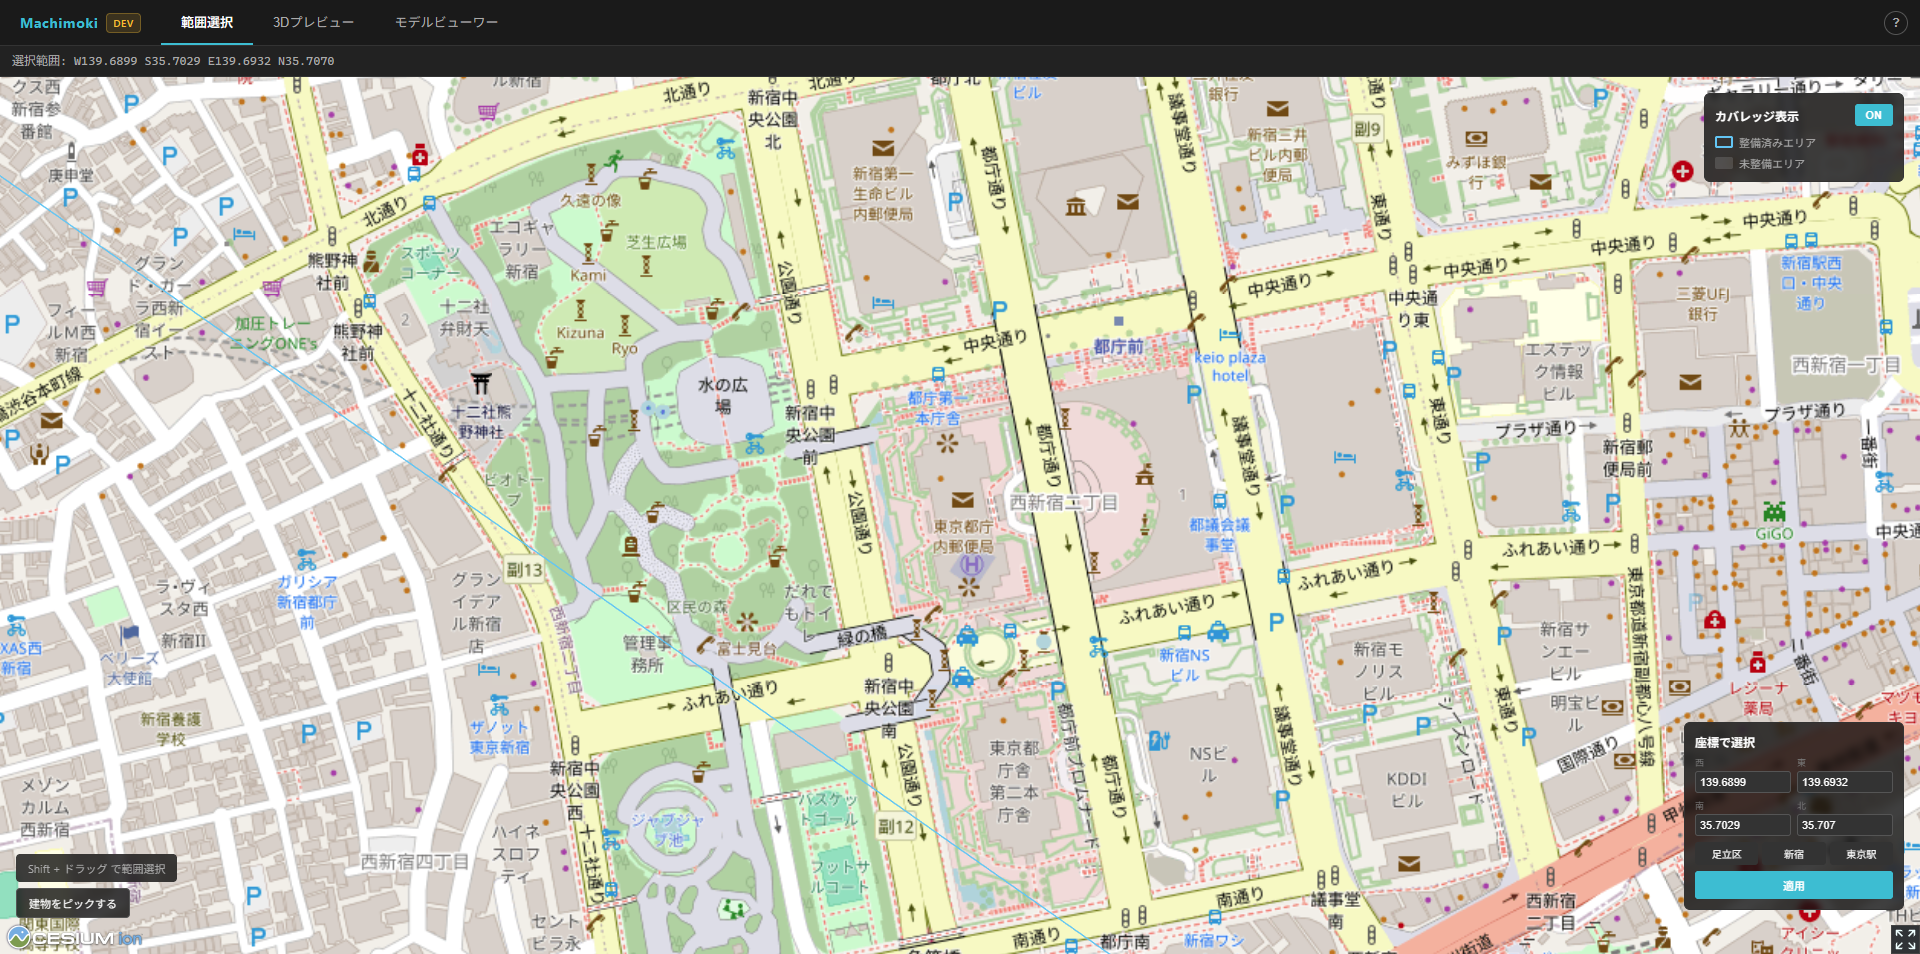
\includegraphics[width=0.78\columnwidth]{machimoki_ui.png}
	\caption{machimoki Webインタフェース：PLATEAUカバレッジ表示と地図上の領域選択}
	\label{fig:ui}
\end{figure}

\section{システム実装}
machimokiは，フロントエンド，コア幾何演算エンジン，バックエンドAPIからなる3層構成で実装した．

\subsection{フロントエンド（Web UI）}
ReactおよびViteを採用し，地図基盤としてCesiumJSとThree.jsを組み合わせている．ユーザーは地理院タイル\cite{gsi}を重畳した地図上で，希望する街区を矩形選択できる（図\ref{fig:ui}）．PLATEAUの整備カバレッジ範囲をオーバーレイ表示し，データが存在する地域を即座に視認可能である．選択領域の建物・地形はThree.jsにより瞬時に3Dプレビュー表示され，模型サイズ，縮尺，地形底面厚み，底面フラット化パラメータをリアルタイムに調整できる．

\subsection{幾何演算パイプラインと品質検証}
メッシュ生成・修復処理は，WebAssembly版の\verb|manifold-3d|\cite{manifold3d}を用いて高速・堅牢に実行される．パイプラインは，(1)~WGS84座標系の矩形範囲正規化，(2)~PLATEAU 3D TilesからのglTF取得と接地輪郭に基づく底面キャッピング，(3)~標高データの64×64格子サンプリングによる底面フラット地形生成，(4)~manifold-3dを用いた建物群と地形メッシュのブール結合（Union），からなる．

生成メッシュに対し，オープンエッジ数，非多様体エッジ数，自己交差数，接続シェル数を自動算出し，完全なソリッド（閉じた立体）であることを確認した上でSTLまたは3MF形式で出力する．3MF形式では建物と地形を色情報付き別オブジェクトとして保持でき，マルチカラー印刷やパーツ分割に最適化される．さらに，モデルとメタデータをZIP形式でまとめた独自コンテナ形式（\verb|.machimoki|）のエクスポートにも対応している．

\section{ユースケースと制作例}
Data Physicalizationのユースケースとして以下のプロトタイプを制作・検証した．

\subsection{防災情報の立体可視化（浸水深シミュレーション）}
新宿駅周辺街区を1/2000スケールで3Dプリントした．建物の内部を中空化し，底部にフルカラーLED（WS2812B）を埋め込んだ．PLATEAUの浸水想定区域データと連動させ，降雨シナリオに応じた浸水水位の上昇を，模型の建物が青から赤へと発光色を変化させることで立体的に表現した．2D地図に比べ，地形の高低差とビル群の浸水リスクが直感的に把握でき，避難ビルへの誘導経路の把握性が向上することを確認した．

\subsection{環境センシング模型と相互連動インタラクション}
大学キャンパス周辺街区模型を制作し，模型内に温度・湿度・照度センサを配置した．マイコン（ESP32）を介してセンサ値をWebサーバへ送信し，Web画面上の3D地図と物理模型の間で相互連動させた．模型上の建物を選択すると画面上で属性情報が表示され，逆に画面上でシミュレーションを実行すると模型のLEDが連動発光する．制作した実物街模型，内蔵LED制御モジュール，およびWeb UIを統合し，任意の街区モデル生成から物理模型上の発光までの一連の相互連動が円滑に機能することを確認した．


\section{まとめ}
本稿では，PLATEAUデータから3Dプリント可能なソリッド模型を生成し，物理デバイス化を支援するツールキット「machimoki」を提案した．Webベースの直感的なUI，manifold-3dを用いた堅牢なソリッド化パイプライン，品質自動検証，フィジカルコンピューティング向け出力を実現した．今後は，配線ダクトや電子部品ソケットの自動生成機能，および多様なセンサとの連携拡充を進める．


\section*{謝辞}
本研究は国土交通省Project\\PLATEAUの都市モデル，国土地理院の地図データを利用した．関係各位に感謝する．



{\small
\bibliographystyle{jwiss}
\bibliography{references}
}

\end{document}
